
\section{Task B}
The agent is an object with a finite set of rules that will move around the
environment.  Our simple reflex agent requires the assumption that the
environment is a rectangular shape, surrounded by walls and free of obstacles.

We've also contemplated an algorithm that will recursively move around the
environment and mark the visited cells to avoid an endless loop situation.

The problem with the recursive algorithm is that the agent has to manage the
counters and initiate the performance calculation itself.

\subsection{Agent}
The agent has the following attributes, some are not used during the algorithms
but will be needed for other types of algorithmic designs. See figure
\ref{fig:agent_uml} for the uml description of bot attributes and functions.

\begin{figure}[h] \label{fig:agent_uml}	\centering
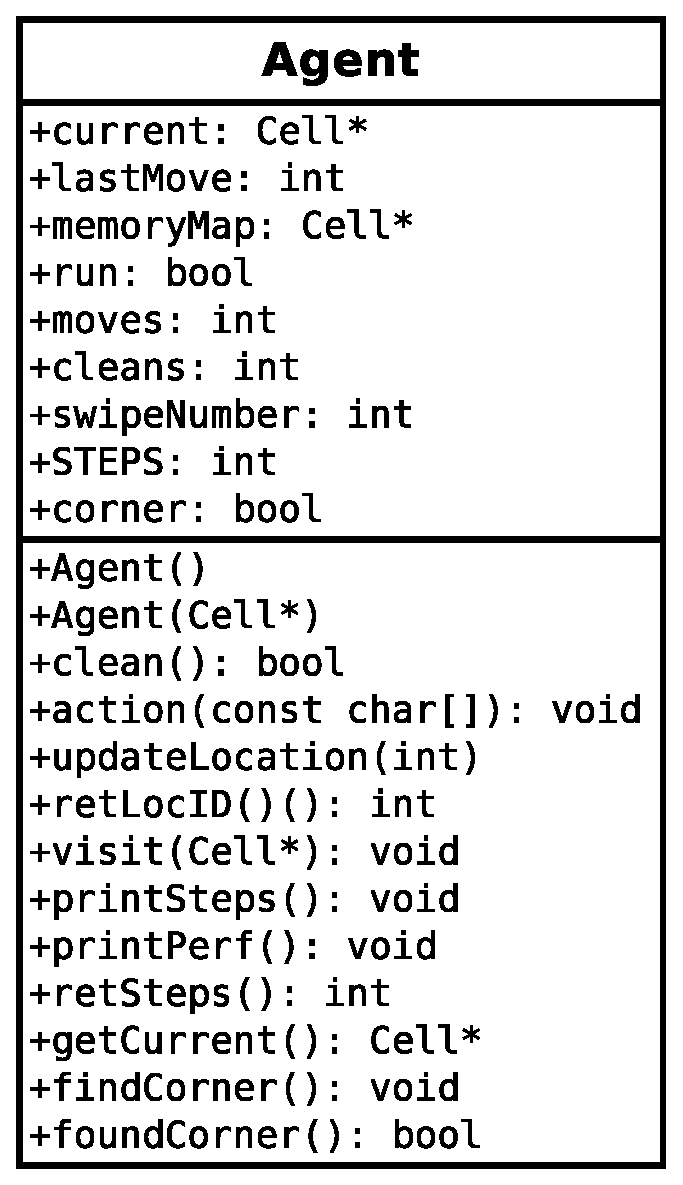
\includegraphics[width=0.3\textwidth]{agent_um}
\caption{UML description of an Agent object}
\end{figure}

\begin{description}
\item[current:]
	This is a Cell* pointer which will point to the current location of the agent.
	Whenever the agent moves the "current" attribute has to be changed to point to
	the new Cell object, which is done by calling the current locations getNeighbor
	function which returns the Cell* pointer to its neighbor.
\item[lasMove:]
	This is an integer describing the direction of the last move made. The moves
	possible are described as a global ENUM as "LEFT", "RIGHT", "UP" and "DOWN".
	By utilizing this the agent can avoid going back to its previous location,
	unless nessecary
\item[memoryMap:]
	This is not currently in use, but can be used to start building a map of the
	environment inside the robots head.  This is set as a Cell, but should be made
	into a different object type with minimal information.
\item[run:]
	This is a boolean value which could  be used to make the agent power down and
	stop cleaning/moving.  Which could be usefull if the room will never get dirtu
	again, since it could stop when finding the second corner.
\item[moves:]
	This is a counter which counts how many movements the agent has performed
	during its run.  This is used when displaying the performance rate of the
	agent.
\item[cleans:]
	This is a counter of how many cells the agent has cleaned during its run. The
	attribute is used during display of the performance rate.
\item[swipeNumber:]
	This is an integer that describes which way the agent is supposed to move.
	The agent will increment this counter each time it hits a wall and thereby
	switch moving to a side. 
\item[STEPS:]
	This is an internal counter to count the number of times the agent has
	perfomed an operation and is used to stop the agent after a certain amount of
	operations.  The counter is for creating an equal amount of movements during
	performance testing.
\item[corner:]
	This is an boolean value describing whether or not the corner has been found.
	The value is set to false during initation and true when the corner is found.
	By utilizing this we can switch from performing the find  corner algorithm to
	our movement algorithm.
\end{description}

\subsection{Two cell environment}
This is the base test for running our agent in an environment.  The environment
is two cells, cell A and B. These cells links to each other and the main running
function controls the agents movements in the following manner. If the agent is
still running, it will start checking if the current cell is clean and clean it
if nessecary.  If it is clean it will check if the left neighbor exists and move
there if it does.  If the left neighbor is non-existant it has hit the end and
should start going to the opposite side. Thus we change the way to move and it
starts moving to the right. When it hits the end of the right cell it will stop
the agent from running or pause it untill it is restarted or the current
location becomes dirty.

To optimize the test case one could check each neighbor of the current location
to see wether it is at the left or right end and then possibly improve the
performance.

Performance is counted by awarding one point for each clean cell at the end of
each step.  It is also seen in context to the amount of movements and the amount
of times the agent cleans a location.

\subsubsection{Non-update performance test}
This performance test was to test the very simple algorithm for two neighboring
cells, which did not become dirty after being cleaned.  We ran each test two
times for each type of initial state. The states was [clean, clean],
[clean,dirty], [dirty,clean], [dirty,dirty].  For each of these states we ran
the test starting in cell A and cell B.

\begin{longtable}{p{0.05\textwidth} p{0.075\textwidth} p{0.075\textwidth} 
									p{0.05\textwidth} p{0.075\textwidth} p{0.075\textwidth} 
									p{0.13\textwidth}}
Start	& A & B & Steps & Moves & Cleans & Performance \\\hline
A & Clean & Clean & 1000 & 1 & 0 & 2000 \\
B & Clean & Clean & 1000 & 2 & 0 & 2000 \\
A & Dirty & Clean & 1000 & 1 & 1 & 2000 \\
B & Dirty & Clean & 1000 & 2 & 1 & 1999 \\
A & Clean & Dirty & 1000 & 1 & 1 & 1999 \\
B & Clean & Dirty & 1000 & 2 & 1 & 2000 \\
A & Dirty & Dirty & 1000 & 1 & 2 & 1998 \\
B & Dirty & Dirty & 1000 & 2 & 2 & 1998 \\
\end{longtable}


\subsubsection{Random dirt performance test}
This test case is the same as previous, but here the environment will receive
randomly generated dirt at the start of each step before the agent perceives the
location.  Then if it has covered all the cells, it will stop and wait for
a maximum of 3 steps or until its current location becomes dirty. Then it will
restart it self and go over the environment once more. This continues until the
number of steps has reached the maximum amount.  They stay very similar because
of the RNG-method chosen. Which is using the ctime library, seed the RNG with
time(0), and generate a random number which is limited with modulus 5.

Each test is run three times to yield some comparison of its randomized dirt
generation.

\begin{longtable}{p{0.05\textwidth} p{0.075\textwidth} p{0.075\textwidth} 
									p{0.05\textwidth} p{0.075\textwidth} p{0.075\textwidth} 
									p{0.13\textwidth}}
Start	& A & B & Steps & Moves & Cleans & Performance \\\hline
A & Clean & Clean & 1000 
		 & 239 & 279 & 1480 \\
	&&&& 233 & 305 & 1404 \\
	&&&& 241 & 292 & 1423 \\
	&&&& 238 & 287 & 1378 \\
	&&&& 231 & 309 & 1426 \\\hline
  &&& AVG & 236.4 & 294.4 & 1422.2\\\hline

B & Clean & Clean & 1000 
		 & 236 & 279 & 1437 \\
	&&&& 236 & 317 & 1412 \\
	&&&& 236 & 306 & 1412 \\
	&&&& 240 & 290 & 1478 \\
	&&&& 244 & 308 & 1474 \\\hline
  &&& AVG & 238.4 & 300.0 & 1442.6 \\\hline
\end{longtable}


\subsection{Simple algorithm}
	This algorithm is good for simple environment shapes, squares or rectangles without many obstacles inside.
	
	The algorithm starts by placing the agent in the bottom left corner, as shown on the picture. 
	By doing this we are certain of the position of the agent and it can move more conciusly.
	This part of the algorithm is pretty simple, the agent when created will only move towards the bottom.
	Once it hits the wall and retreats it will only go to the left.
	Again, when the left wall is hitted the agent knows its exact location.
	This part of the algorithm is only done the first time it executes.
	Once it finds the bottom left corner once its enough.

\begin{figure}[h] \label{fig:corner}	\centering
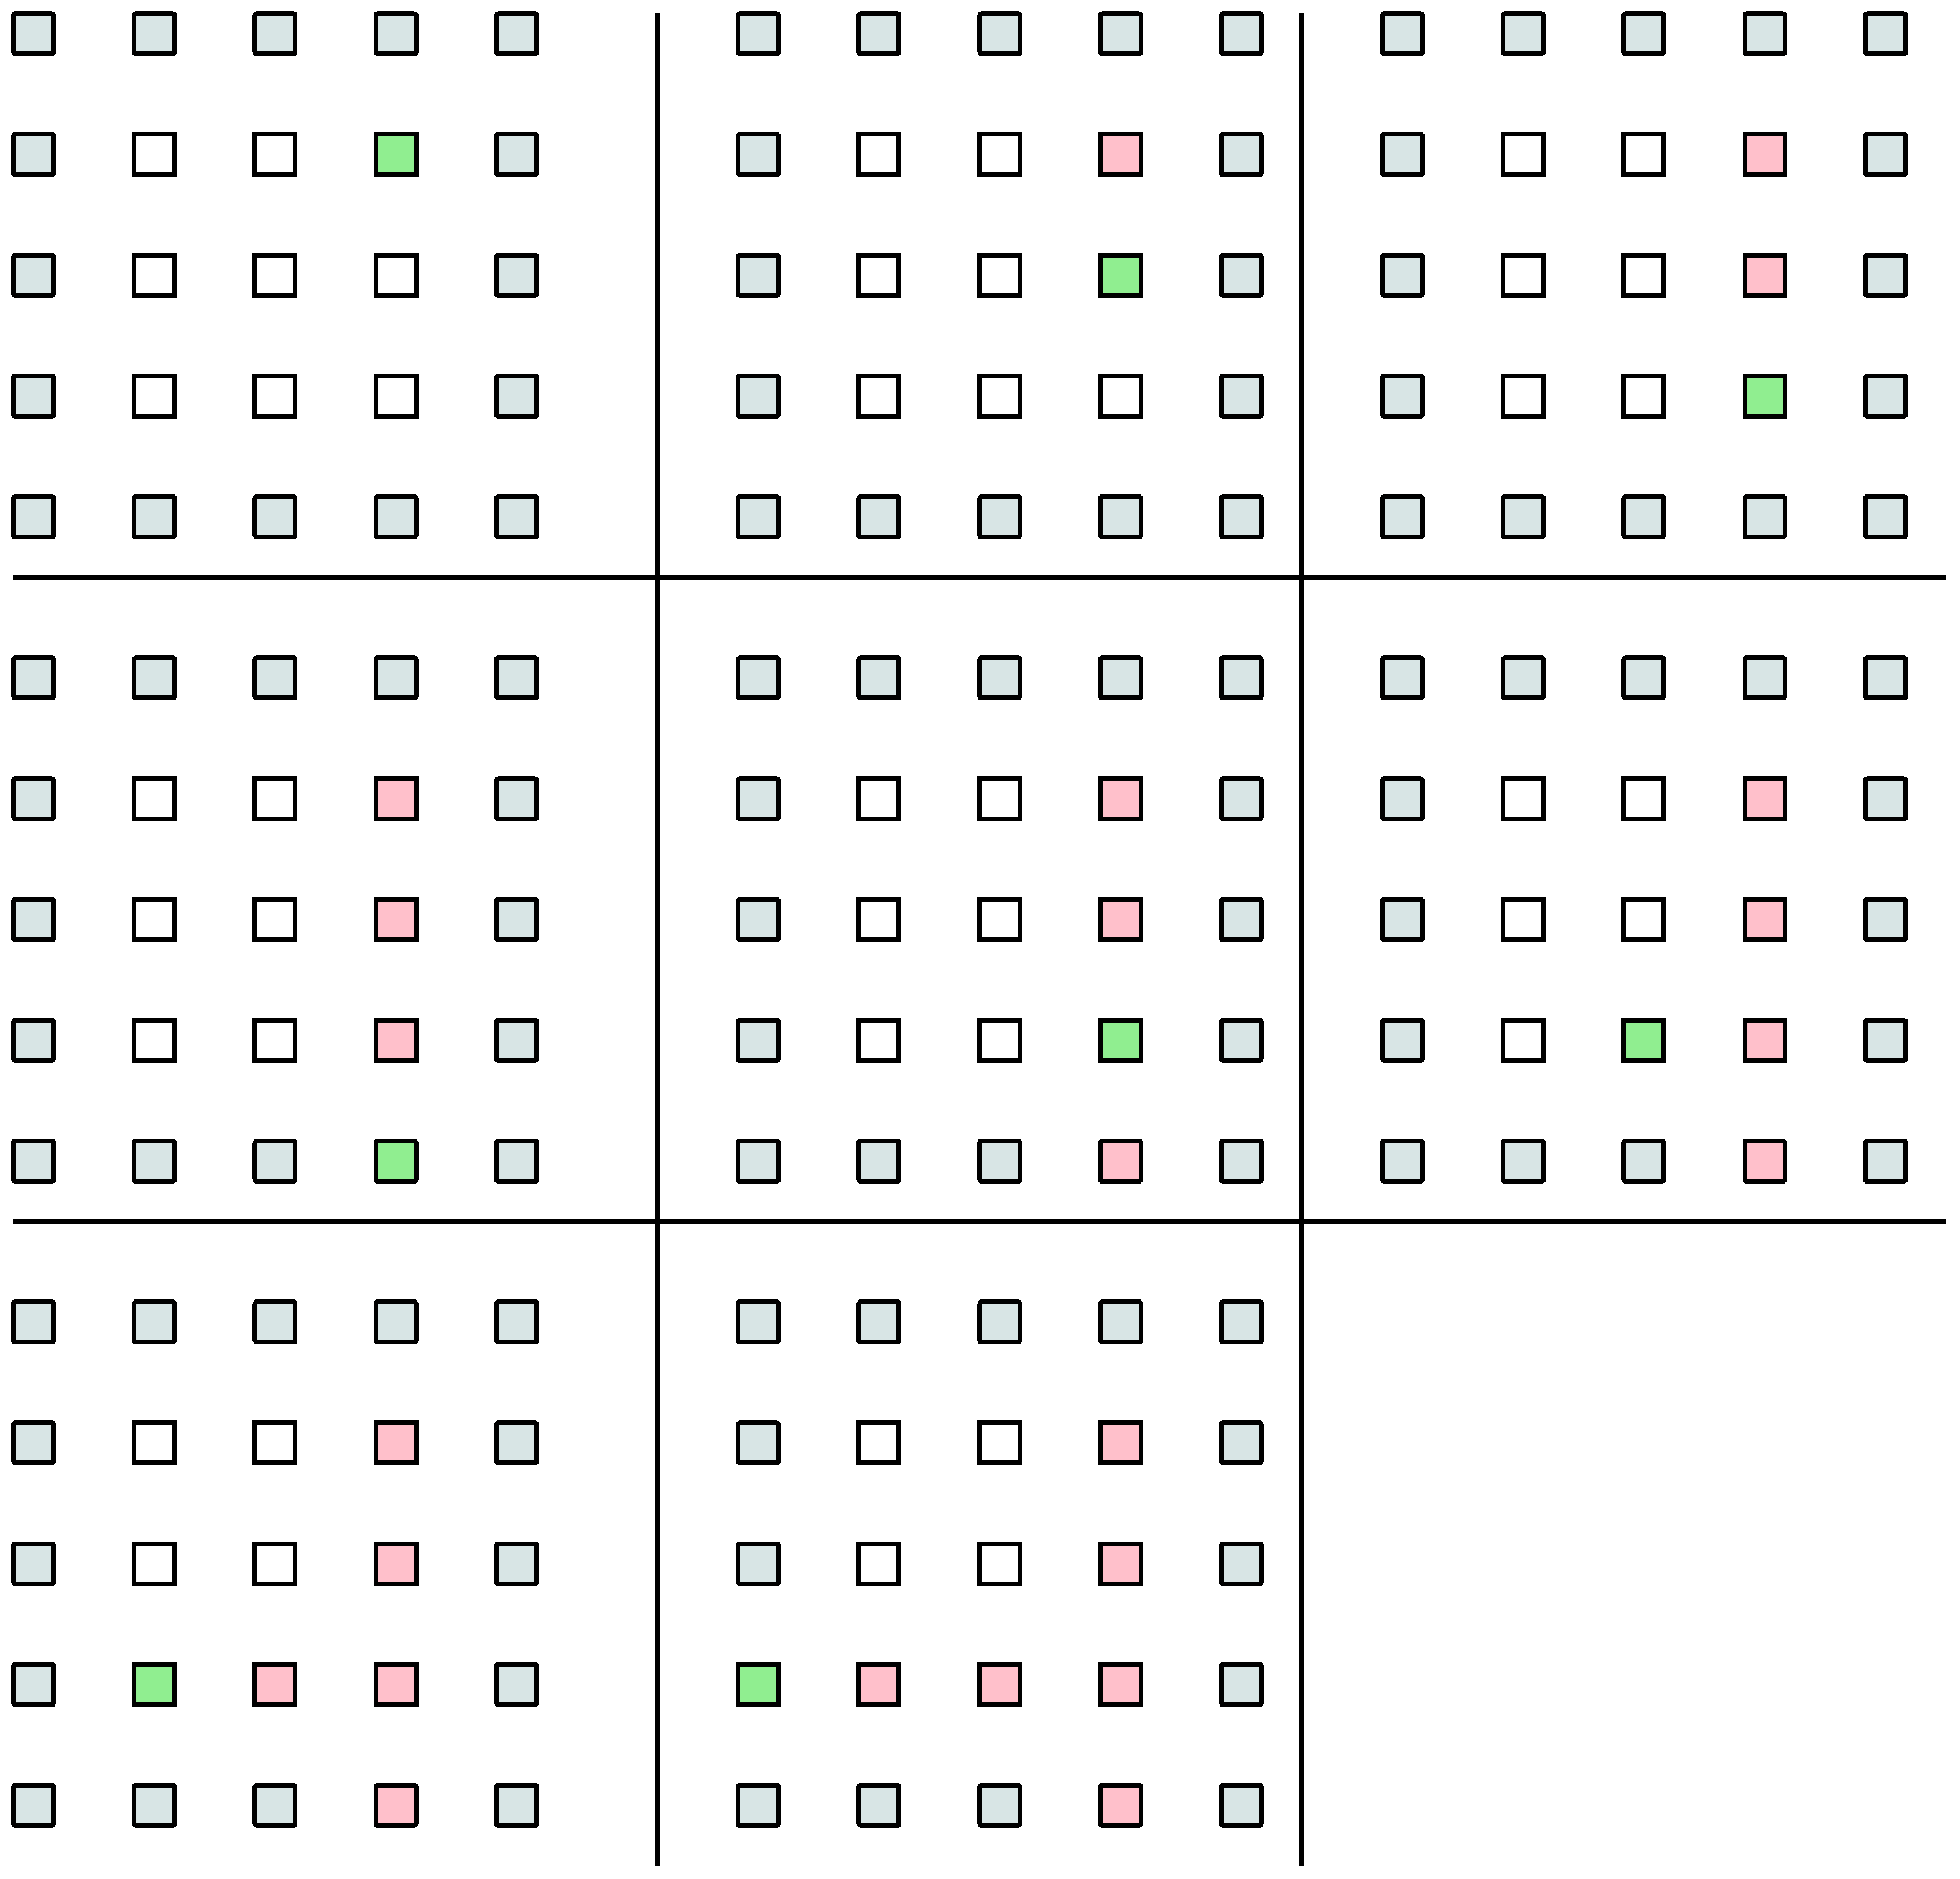
\includegraphics[width=0.5\textwidth]{find_corner}
\caption{How the agent finds the corner}
\end{figure}

After finding the bottom left corner the agent starts the actual algorithm. The
algorithm moves the agent in an S shape. Being in the bottom left corner the
agent will start the first swipe to the right in the first row.	Once the agent
hits the bottom right corner the agent will move one row up, and start the swipe
number 2, to the left.	The variable swipeNumber is used to control in which
direction the agent should go.	If the swipeNumber is an odd number the agent
moves to the right until it find the wall. If it's an even number it moves to
the left.	When the agent hits the top wall it starts going down to find the
bottom row.	Once in the bottom row the number of swipes is increased again and
the agent starts again the algorithm.	In the figure is easy to see how the agent
moves, each of the red lines will be a movement and the green lines are the
reaction of the agent after finding a wall.


\begin{figure}[h]\label{fig:simpleAlgorithm} \centering
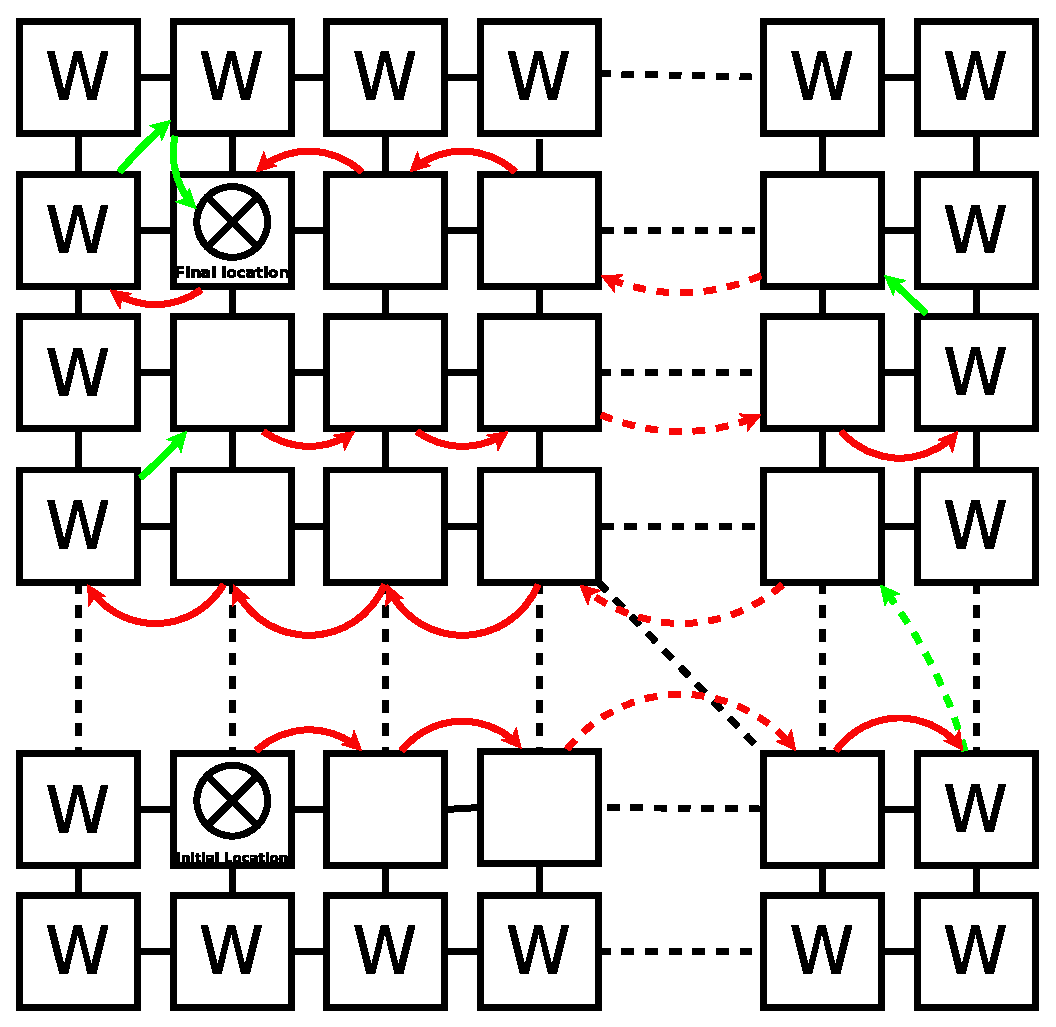
\includegraphics[width=0.5\textwidth]{SimpleAlgorithm}
\caption{How the agent moves}
\end{figure}


\begin{longtable}{p{0.05\textwidth} p{0.075\textwidth} p{0.075\textwidth} 
									p{0.05\textwidth} p{0.075\textwidth} p{0.075\textwidth} 
									p{0.13\textwidth}}
Start	& A & B & Steps & Moves & Cleans & Performance \\\hline
A & Clean & Clean & 1000 
		 &  &  &  \\
	&&&&  &  &  \\
	&&&&  &  &  \\\hline
  &&&  AVG &  &  &  \\\hline
b & Clean & Clean & 1000 
		 &  &  &  \\
	&&&&  &  &  \\
	&&&&  &  &  \\\hline
  &&&  AVG &  &  &  \\\hline
\end{longtable}


\subsection{Harder algorithm}


\begin{figure}[h] \label{fig:}	\centering
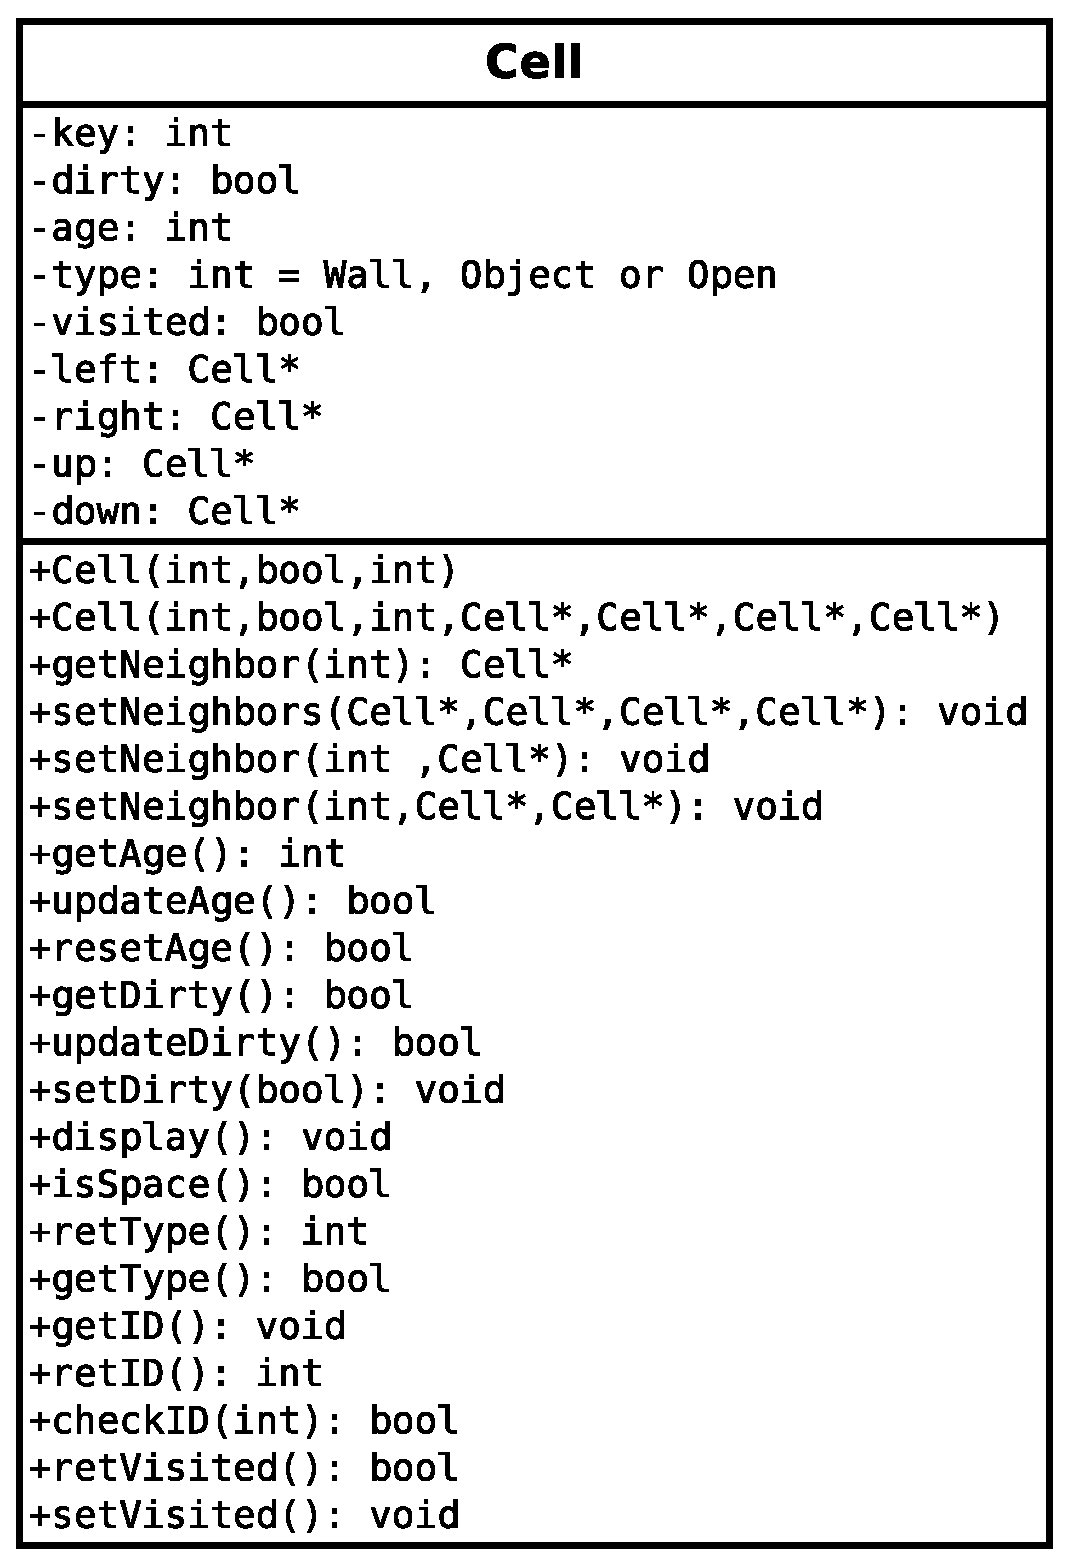
\includegraphics[width=0.3\textwidth]{cell_uml}
\caption{}
\end{figure}

\begin{figure}[h] \label{fig:}	\centering
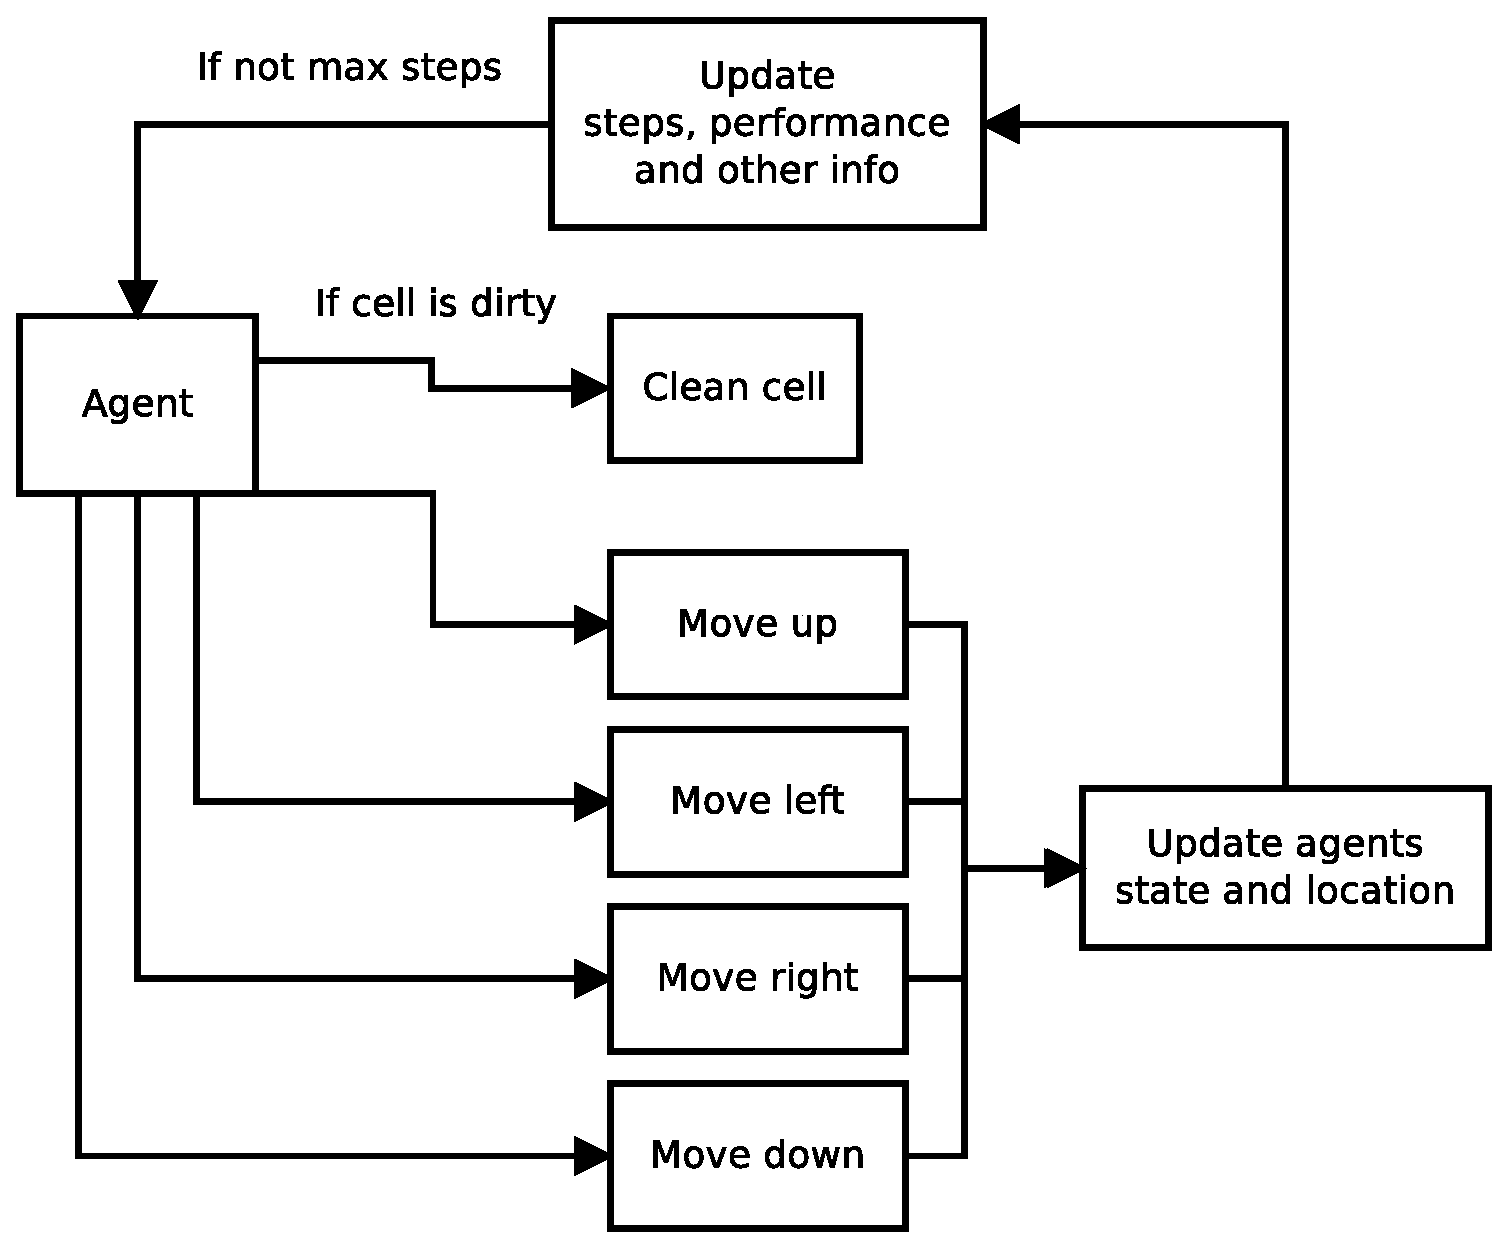
\includegraphics[width=0.5\textwidth]{agent}
\caption{}
\end{figure}

\begin{longtable}{p{0.05\textwidth} p{0.075\textwidth} p{0.075\textwidth} 
									p{0.05\textwidth} p{0.075\textwidth} p{0.075\textwidth} 
									p{0.13\textwidth}}
Start	& A & B & Steps & Moves & Cleans & Performance \\\hline
A & Clean & Clean & 1000 
		 &  &  &  \\
	&&&&  &  &  \\
	&&&&  &  &  \\\hline
  &&&  AVG &  &  &  \\\hline
b & Clean & Clean & 1000 
		 &  &  &  \\
	&&&&  &  &  \\
	&&&&  &  &  \\\hline
  &&&  AVG &  &  &  \\\hline
\end{longtable}


